\documentclass[14pt]{extreport}

% Основные пакеты
\usepackage[english, russian]{babel}    % Поддержка русского и английского языков
\usepackage{graphicx}                   % Для вставки изображений
\usepackage{import}                     % Для продвинутого импорта (например, pdf_tex из Inkscape)
\usepackage{subcaption}                 % Для создания подписей к фигурам
\usepackage{float}                      % Для улучшенного позиционирования фигур
\usepackage{geometry}                   % Для управления отступами на странице
\usepackage{amsmath}                    % Для расширенной поддержки математики
\usepackage{amsfonts}                   % Математические шрифты
\usepackage{amssymb}                    % Математические символы
\usepackage{tabu}                       % Улучшенные таблицы
\usepackage{booktabs}                   % Профессиональные таблицы с вертикальными разделителями
\usepackage[dvipsnames]{xcolor}         % Расширенная поддержка цветов
\usepackage{longtable}                  % Для таблиц, занимающих несколько страниц
\usepackage{makecell}                   % Для улучшенного форматирования ячеек таблиц
\usepackage{multirow}                   % Для объединения строк в таблицах
\usepackage{tabularray}                 % Для современных таблиц
\usepackage{varwidth}                   % Для переменной ширины блоков
\usepackage{hyperref}                   % Для гиперссылок
\usepackage{verbatim}                   % Для вставки кода
\usepackage{listings}                   % Для оформления листингов кода
\usepackage{amsmath}
% Настройка графики
\graphicspath{ {./images/} }            % Путь к папке с изображениями

% Настройка отступов на странице
\geometry{left=2cm, right=2cm, bottom=2cm, top=2cm}

% Настройка гиперссылок
\hypersetup{
    linkcolor=blue,                     % Цвет ссылок
    filecolor=magenta,                  % Цвет ссылок на файлы
    urlcolor=cyan                       % Цвет URL-адресов
}

\definecolor{codegreen}{rgb}{0,0.6,0}  % Цвет для комментариев
\definecolor{codegray}{rgb}{0.5,0.5,0.5}  % Цвет для номеров строк
\definecolor{codepurple}{rgb}{0.58,0,0.82}  % Цвет для строк
\definecolor{backcolour}{rgb}{0.95,0.95,0.92}  % Цвет фона

% Определим стиль для выделения переменных
\lstdefinestyle{codestyle}{
    backgroundcolor=\color{backcolour},  % Цвет фона
    commentstyle=\color{codegreen}\itshape,  % Стиль для комментариев
    keywordstyle=\color{magenta}\bfseries,  % Стиль для ключевых слов
    numberstyle=\tiny\color{codegray},  % Стиль для номеров строк
    stringstyle=\color{codepurple},  % Стиль для строк
    identifierstyle=\color{blue},  % Стиль для переменных (выделим их синим)
    basicstyle=\ttfamily\footnotesize,  % Размер шрифта для кода
    breakatwhitespace=false,  % Не разрывать строки в пробелах
    breaklines=true,  % Разбивать длинные строки
    captionpos=b,  % Позиция заголовка (внизу)
    keepspaces=true,  % Сохранять пробелы
    numbers=left,  % Позиция номеров строк
    numbersep=10pt,  % Расстояние между кодом и номерами строк
    showspaces=false,  % Не показывать пробелы
    showstringspaces=false,  % Не показывать пробелы в строках
    showtabs=false,  % Не показывать табуляции
    tabsize=4,  % Размер табуляции
    frame=single,  % Добавить рамку вокруг кода
    rulecolor=\color{black},  % Цвет рамки
    backgroundcolor=\color{backcolour},  % Цвет фона рамки
    xleftmargin=15pt,  % Отступ слева
    xrightmargin=15pt,  % Отступ справа
}


\lstset{style=codestyle}
\lstset{extendedchars=\true}

\begin{document}

\begin{titlepage}
    \centering
    \vspace*{1cm}

    {\large Министерство науки и высшего образования Российской Федерации}\\
    {\large ФЕДЕРАЛЬНОЕ ГОСУДАРСТВЕННОЕ АВТОНОМНОЕ ОБРАЗОВАТЕЛЬНОЕ УЧРЕЖДЕНИЕ ВЫСШЕГО ОБРАЗОВАНИЯ «НАЦИОНАЛЬНЫЙ ИССЛЕДОВАТЕЛЬСКИЙ УНИВЕРСИТЕТ ИТМО»}\\
    {\large (УНИВЕРСИТЕТ ИТМО)}\\

    \vspace{1cm}

    \textbf{{\Huge ОТЧЕТ}\\
    {\Huge О ЛАБОРАТОРНОЙ РАБОТЕ №1}}\\

    \vspace{1cm}

    {\LARGE По дисциплине\\
     \(\lll\) Математическая Статистика \(\ggg\) }\\

    \vspace{2cm}

    {\Large Студенты:}\\
    Охрименко Eва\\
    Даниил Буцкий


    \vspace{2cm}

    {\Large Проверил:}\\
    Шкваренко Андрей Алексеевич\\

    \vspace{2cm}

    {\large г. Санкт-Петербург}\\
    {\large 2025}

\end{titlepage}
\newpage
\tableofcontents
\newpage

\section{Task}

В этом задании нам нужно найти оценку масштабируемого параметра \( \theta^2 \)
методом моментов для распределения Лапласа.

Итак, зададим массив объемов выборки:

\begin{lstlisting}[language=Python, caption={Массив объемов выборок}]
sampleSizes = [i for i in range(10, 1000, 3)]
\end{lstlisting}


А также зададим константы и инициализируем массивы, которые нам потребуются в задании:
За \texttt{theta} обозначен параметр распределения, за \texttt{m} - количество эксперементов для каждой выборки.
\begin{lstlisting}[language=Python, caption={Init}]
theta = 0.5 
trueThetaKvadrat = theta**2
m = 1000 

biases = []
variances = []
mses = []
\end{lstlisting}


Выведем оценку $\theta^2$ методом моментов для распределения Лапласа с плотностью:
\[
f_\theta(x) = \frac{1}{2\theta} \exp\left(-\frac{|x|}{\theta}\right)
\]

\begin{enumerate}
    \item Теоретический второй момент:
    \[
    E[X^2] = \text{Var}(X) = 2\theta^2
    \]
    
    \item Выборочный второй момент:
    \[
    \frac{1}{n}\sum_{i=1}^n x_i^2
    \]
    
    \item Приравниваем моменты:
    \[
    2\theta^2 = \frac{1}{n}\sum_{i=1}^n x_i^2
    \]
    
    \item Оценка параметра:
    \[
    \theta^2 = \frac{1}{2n} \sum_{i=1}^n x_i^2
    \]
\end{enumerate}


Для каждого размера выборки сгенерируем несколько выборок, 
расчитаем для каждой оценку параметра \( \theta^2 \), 
и сохраним результат в списке \texttt{ozenkaTheta}:

\begin{lstlisting}[language=Python, caption={Цикл}]
for i in sampleSizes:
    ozenkaTheta = list()
    for extreptiza in range(m):
        sample = np.random.laplace(loc=0, scale=theta, size=i)

        ozenkaTheta.append(np.sum(sample**2) / (2*i))
\end{lstlisting}

Теперь для каждого размера выборки вычислим смещение оценки, 
 выборочную дисперсию оценок и среднеквадратическую ошибку (MSE), 
 которые затем сохраним для анализа.

 \begin{lstlisting}[language=Python, caption={Расчет}]
    ozenkaTheta = np.array(ozenkaTheta)

    bias = np.mean(ozenkaTheta) - trueThetaKvadrat
    variance = np.var(ozenkaTheta, ddof=1)
    mse = bias**2 + variance

    biases.append(bias)
    variances.append(variance)
    mses.append(mse)
\end{lstlisting}


Теперь нарисуем полученные графики:


\begin{figure}[h]
    \centering
    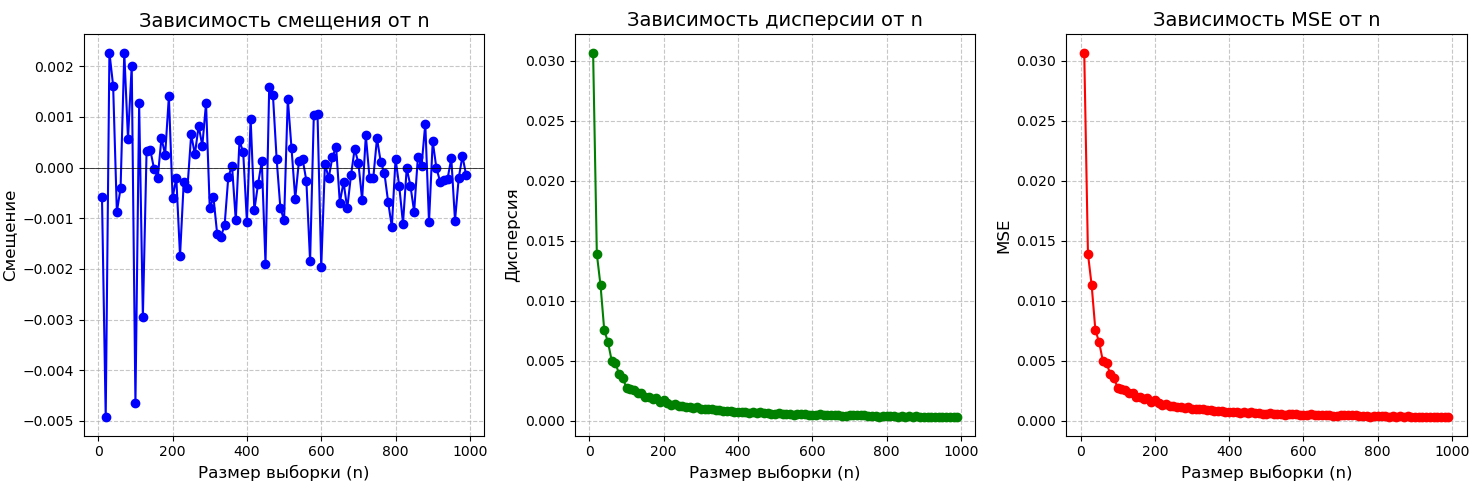
\includegraphics[width=1\textwidth]{image1.png}
    \caption{Графики}
\end{figure}

Итак, можно заметить, что смещение оценки стремится к нулю(это хорошо).
Димперсия, то есть разброс оценок уменьшается, а также сумма квадрата
смещения и дисперсии уменьшается, это дает на понять, что все 3 метрики уменьшаются
с увеличением объема данных.


\end{document}